
\documentclass[draft,linenumbers]{agujournal}\usepackage{knitr}
\usepackage[hidelinks]{hyperref}
\usepackage{amsmath}
% \draftfalse

\journalname{Earth's Future}



%










\IfFileExists{upquote.sty}{\usepackage{upquote}}{}
\begin{document}
\title{Urban Water Conservation Policies in the United States}

\authors{Jonathan M. Gilligan\affil{1,2}, Christopher A. Wold\affil{3}, Scott C. Worland\affil{2}, John J. Nay\affil{2}, David J. Hess\affil{4}, George M. Hornberger\affil{2}}

\affiliation{1}{Department of Earth \& Environmental Sciences, Vanderbilt University, Nashville, Tennessee, USA}
\affiliation{2}{Department of Civil \& Environmental Engineering, Vanderbilt University, Nashville, Tennessee, USA}
\affiliation{3}{Vanderbilt Institute for Energy and Environment, Vanderbilt University, Nashville, Tennessee, USA}
\affiliation{4}{Department of Sociology, Vanderbilt University, Nashville, Tennessee, USA}
% \affiliation{4}{U.S. Geological Survey, Nashville, Tennessee, USA}

\correspondingauthor{Jonathan M. Gilligan}{jonathan.gilligan@vanderbilt.edu}

%% Keypoints, final entry on title page.

% Example:
% \begin{keypoints}
% \item	List up to three key points (at least one is required)
% \item	Key Points summarize the main points and conclusions of the article
% \item	Each must be 100 characters or less with no special characters or punctuation
% \end{keypoints}

%  List up to three key points (at least one is required)
%  Key Points summarize the main points and conclusions of the article
%  Each must be 100 characters or less with no special characters or punctuation

\begin{keypoints}
\item Analysis of water conservation policies of 195 cities in 45 states
\item Water conservation policies correlate with both environmental and social variables
\item Partisan voting patterns at both state and metropolitan levels account for much of the variation
\end{keypoints}

%% ------------------------------------------------------------------------ %%
%
%  ABSTRACT
%
% A good abstract will begin with a short description of the problem
% being addressed, briefly describe the new data or analyses, then
% briefly states the main conclusion(s) and how they are supported and
% uncertainties.
%% ------------------------------------------------------------------------ %%

%% \begin{abstract} starts the second page

\begin{abstract}
Urban water supply systems in the United States are increasingly stressed as economic and population growth confront limited water resources.
Demand management, through conservation and improved efficiency, has long been promoted as a practical alternative to building Promethean energy-intensive water-supply infrastructure. Some cities are making great progress at managing their demand, but study of conservation policies has been limited and often regionally focused. We present a hierarchical Bayesian analysis of a new measure of urban water conservation policy, the Vanderbilt Water Conservation Index (VWCI), for 195~cities in 45~states in the contiguous United States. Cities in states with arid climates and greater tendency to vote for Democratic candidates tend to adopt more conservation measures. Within a state, cities with large and rapidly growing populations and greater propensity than the rest of the state to vote Democratic tend to adopt more conservation measures. Economic factors and climatic differences between cities do not have much effect on the number of measures adopted, but they impact the character of the measures, with arid cities favoring mandatory conservation actions and cities in states with lower real personal income favoring rebates for voluntary actions. Understanding relationships between environmental and societal factors and cities' support for water conservation measures can help planners and policy-makers identify obstacles and opportunities to increase the role of conservation and efficiency in making urban water supply systems sustainable.
\end{abstract}


%% ------------------------------------------------------------------------ %%
%
%  TEXT
%
%% ------------------------------------------------------------------------ %%
\section{Introduction}
Cities face increasing challenges to their water supply because of complex interactions among drought, infrastructure, population growth, land-use changes, and other natural and human factors.
The prospect of climatic change adds to the difficulty of planning robust and sustainable water supply systems, on account both of  increasing uncertainty about future supply and demand for water, and also of predicted reductions in water availability in some regions, such as the Southwestern United States \citep{gcrp_natl_assessment_3_2014}.
For many years, advocates of soft approaches to managing water resources have stressed the importance of improving the efficiency with which society obtains the water services it requires \citep{gleick_soft_water_paths_2002}.
Some cities and their associated water-supply systems respond to these challenges by pursuing grand energy-intensive infrastructure projects to draw water from distant or difficult sources, but many have also shown increasing interest in the soft path, managing demand through efficiency and conservation measures, and a number of cities have made impressive progress \citep{fleck_fighting_2016}.

A pressing challenge is to identify the characteristics of successful transitions toward sustainable water use and the necessary conditions for those transitions to spread more widely.
Studies have investigated urban water conservation policies and several water conservation indices are available, but these either lack comprehensive coverage of water conservation policies or are geographically limited \citep{hess_vwci_2017,sauri_conservation_2013,maggioni_conservation_2014}.
Recent research finds that individual perception of water scarcity and preference for policy action to address scarcity depend not only on the actual degree of water scarcity, but also on the person's ideological worldview \citep{switzer_green_lenses_2016}, but it is not clear how these individual preferences translate into policy action.

The Vanderbilt Water Conservation Index (VWCI) is an integer score representing the number of measures that a city has taken to reduce its water demand, out of a list of 79 possible policy actions \citep{hornberger_water_conservation_2015, hess_drought_2016, hess_vwci_2017}.
This list includes 31 requirements, such as restrictions on lawn-watering or mandatory use of water-efficient plumbing in new construction and renovations; and 21 rebates offered for voluntary actions, such as purchasing water-efficient appliances.
Previously, we assessed this index and performed preliminary quantitative and qualitative analyses on a subset of the 22 central cities of the largest metropolitan statistical areas (MSAs) in the extended Southwestern United States \citep{hess_drought_2016}.

Our preliminary analysis of the 22~largest MSAs in the Southwest found that propensity to adopt water conservation measures depended both on characteristics of the physical environment (precipitation) and socio-economic and political characteristics of the MSA (partisan voting and cost of living). The Cook Partisan Voting Index for an MSA had, by a large margin, the greatest predictive power for adopting water conservation measures. This finding was supported by qualitative analysis, which suggested that political association of water conservation with general ``environmentalist'' politics created political differences in the ways that cities respond to the physical fact of water scarcity.

We subsequently expanded our database to the central cities in 197~MSAs in 47 states \citep{hess_vwci_2017}, which comprise more than half of the 382~MSAs in the United States \citep{census_population_2015} and here, we present the first quantitative analysis of the larger database, analyzing relationships between environmental and societal characteristics of 195~cities across the contiguous United States and those cities' propensity to adopt water conservation policies. This analysis considers state-level as well as MSA-level variables. We identify which variables best explain variations in water conservation policy regimes, how effects at the state level moderate city-level effects, and whether these effects manifest differently when we consider specific aspects of water-conservation policy, such as requirements and rebates.
%We find that differences in climate, political leanings of voters, and  demographics are reflected in the number and kind of water conservation measures adopted by U.S. cities. Such insights
This analysis may help water managers and policy makers to anticipate how receptive a given city might be to adopting different conservation measures.

\section{Data and Methods}
\label{sec:data.methods}
\subsection{Vanderbilt Water Conservation Index}
%
% vwci_histogram figure
%
% jg_tex_chunk_hook

\begin{figure}[tb]

{\centering 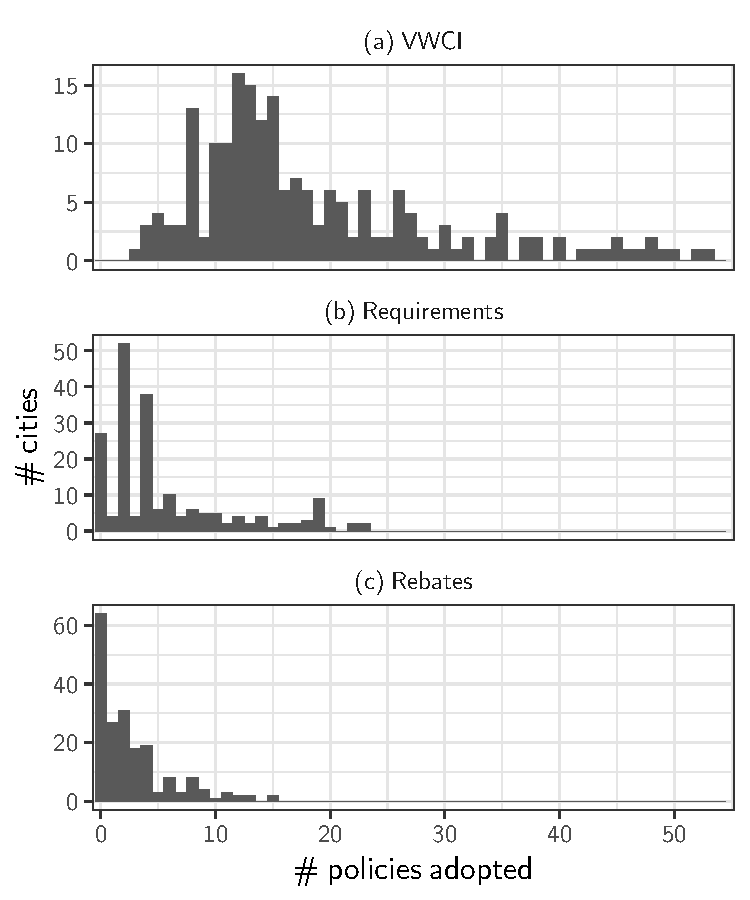
\includegraphics[width=0.8\linewidth]{figure/vwci_histogram-1}

}

\caption[Distribution of VWCI, requirements, and rebates]{Distribution of VWCI, requirements, and rebates.}\label{fig:vwci_histogram}
\end{figure}


%The VWCI data set provides detailed information about both the number and nature of water conservation policies in n_all_cities ~cities in n_all_states~states  \citep{hess_drought_2016,hess_vwci_2017}.
The full VWCI data set provides detailed information about both the number and nature of urban water conservation policies, which  allows hierarchical analysis to examine the relationships between water conservation scores and hydroclimatological and societal characteristics at both state and MSA levels.
Our complete database includes Anchorage, AK, and Honolulu, HI, but for this analysis we chose to include only cities within the contiguous United States (195~cities in 45~states, Fig~S1)  because both climatic and socio-political characteristics of Alaska and Hawaii may be very different from those of the contiguous states, and also because state-level variables that average over the enormous area of Alaska and across the multiple Hawaiian islands may render them less suitable for our hierarchical treatment.

VWCI scores range from~3 to~53 with a mean of 18.7 and a median of 15 (Figure~\ref{fig:vwci_histogram}a; Table~S1). The number of requirements ranges from  from~0 to~23 with a mean of 5.6 and a median of 4 (Figure~\ref{fig:vwci_histogram}b) and the number of rebates ranges from~0 to~15 with a mean of 2.7 and a median of 2 (Figure~\ref{fig:vwci_histogram}c).
%
% set_top_vwci_count
%

%
% top_vwci table
%
% latex table generated in R 3.3.3 by xtable 1.8-2 package
% Mon Apr  3 17:22:23 2017
\begin{table}[tbp]
\centering
\caption{Cities with the twenty highest VWCI scores. Req. = requirements, Reb. = rebates. A complete list of all  195  cities appears in Table~S1.}
\label{tab:top_vwci}
\begin{tabular}{rlrrrr}
  \hline
\multicolumn{1}{c}{ Rank } & \multicolumn{1}{c}{ City } & \multicolumn{1}{c}{ VWCI } & \multicolumn{1}{c}{ Req. } & \multicolumn{1}{c}{ Reb. } & \multicolumn{1}{c}{ $\text{Req.}/\text{Reb.}$ } \\
  \hline
  1 & Los Angeles, CA &  53 &  23 &  13 & 1.77 \\
    2 & San Diego, CA &  52 &  19 &  15 & 1.27 \\
    3 & Santa Rosa, CA &  50 &  19 &  15 & 1.27 \\
    4 & Oxnard, CA &  49 &  23 &  11 & 2.09 \\
    5 & San Jose, CA &  48 &  22 &  12 & 1.83 \\
    5 & Santa Cruz, CA &  48 &  20 &  11 & 1.82 \\
    7 & Austin, TX &  47 &  19 &  11 & 1.73 \\
    8 & San Antonio, TX &  46 &  19 &   8 & 2.38 \\
    9 & Albuquerque, NM &  45 &  19 &  12 & 1.58 \\
    9 & Riverside, CA &  45 &  15 &  13 & 1.15 \\
   11 & Fresno, CA &  44 &  22 &   8 & 2.75 \\
   12 & Denver, CO &  43 &  19 &   8 & 2.38 \\
   13 & San Francisco, CA &  42 &  18 &   9 & 2.00 \\
   14 & Las Vegas, NV &  40 &  18 &   7 & 2.57 \\
   14 & Salinas, CA &  40 &  19 &   6 & 3.17 \\
   16 & El Paso, TX &  38 &  19 &   3 & 6.33 \\
   16 & Miami, FL &  38 &  14 &   8 & 1.75 \\
   18 & Fort Collins, CO &  37 &   9 &   8 & 1.12 \\
   18 & Stockton, CA &  37 &  14 &   8 & 1.75 \\
   20 & New York, NY &  35 &  19 &   2 & 9.50 \\
   20 & Salt Lake City, UT &  35 &  18 &   2 & 9.00 \\
   20 & Tampa, FL &  35 &  14 &   5 & 2.80 \\
   20 & Vallejo, CA &  35 &  14 &   6 & 2.33 \\
   \hline
\end{tabular}
\end{table}

The 20~cities with the greatest VWCI scores are in states in the Western U.S., with the exception of two cities in Florida and one in New York (Tables~\ref{tab:top_vwci}, S1). Cities with similar total VWCI scores, such as New York and Salt Lake City vs.\ Tampa and Vallejo, El Paso vs.\ Miami, and Riverside vs.\ Fresno, may have very different relative contributions from requirements and rebates.

The relative contributions of rebates and requirements to VWCI varied considerably (Table~\ref{tab:top_vwci}), and our previous qualitative research indicated that there might be a preference for rebates over requirements in more politically conservative cities \citep{hess_drought_2016,brown_politics_2016}. Consequently, in addition to the VWCI score we also analyzed the number of rebates and the number of requirements in a city's portfolio of conservation policies.

\subsection{Explanatory Variables}
We obtained values for the MSA-level average annual average temperature ($T$) and total precipitation ($P$) for the period 1970--2014 from the University of Delaware's gridded climate reanalysis \citep{matsuura_gridded_temp_2015,matsuura_gridded_precip_2015} and for state-level from the National Climatic Data Center's divisional temperature and precipitation records for the Continental U.S. \citep{vose_nclimdiv_2014}.
% PDSI was calculated from temperature and precipitation using a MATLAB software
% package by Jacobi \emph{et al.} and the historical drought severity was
% calculated as the longest run of consecutive years from 1900--2010 with
% $\text{PDSI} \le -3$ \citep{jacobi_PDSI_2015}.
We obtained populations for MSAs and states in 2010 and 2014 from the \citet{census_population_2015} and used them to calculate average annual rates of population growth.
Per-capita real personal income (RPI) for MSAs and states in 2014  were was obtained from the \citet{bea_rpi_2016}.
The fraction of the public water supply taken from surface water sources (henceforth, surface-water fraction) was obtained from the U.S. Geological Survey's water use report for 2010 \citep{maupin_water_use_2014}.
The Cook Partisan Voting Index (PVI) was calculated using state- and county-level presidential votes, averaged over the 2008 and 2012 elections \citep{cook_pvi_2013, cq_elections_2016}. Positive PVI indicates a greater Democratic vote share than the national average and negative PVI a greater Republican vote share (Tables~S1--S2 and Datasets~S1--S2).

We began with the covariates listed above, but adopted a modified set based on preliminary results: The regression coefficients for $T$ and $P$ showed collinearity.
This, together with a desire for parsimony, led us to replace them with the K\"oppen aridity index: $P / (T + 33)$, with $P$ in millimeters and $T$ in Celsius.
The K\"oppen index is deemed an especially reliable index of aridity \citep{quan_aridity_2013}. Larger values of this index correspond to wetter conditions and smaller values to drier conditions.

The distribution of MSA population in~2014 was skewed, with a few large cities producing an asymmetric fat tail (Figure~S2), so we deemed natural logarithm of population more suitable for a regression analysis \citep[pp.~59--61]{gelman_arm_2007}.

\subsection{Regression Analysis}
We applied Bayesian hierarchical varying-intercept regression to each of the three conservation scores (VWCI, number of requirements, and number of rebates) with the following explanatory variables: the K\"oppen aridity index, surface water fraction, PVI, RPI, metropolitan population, and population growth rate. The hierarchical structure of our regression model, which nests cities and MSAs within states, reflects the fact that water resources extend beyond MSA boundaries and that state-level policies affect local actions, both by constraining local ordinances and regulations, and by encouraging or requiring counties and cities to adopt various types of conservation measures.

The regression models each city's conservation score (VWCI, requirements, or rebates) as the result of a beta-binomial process (an overdispersed analogue to a binomial process) \citep[pp.~437--38]{gelman_bda_2014}.
This model characterizes each city $i$ by a probability $p_i$ for adopting water conservation policies. In a pure binomial process, each policy would have the same probability $p_i$ of being adopted in city $i$, but the beta-binomial process allows for greater dispersion of scores by drawing the probability for each action separately from a beta distribution with mean $p_i$.
The probability $p_i$ is modeled using a hierarchical varying-intercept logistic regression on both state-level and MSA-level covariates:
\begin{linenomath*}
\begin{align}
\text{Score}_i \sim{}& \text{beta-binomial}(N_{\text{action}}, \phi p_i, \phi (1 - p_i)), \\
\intertext{where}
p_i ={}& \text{logit}^{-1}(y_i),\\
y_i ={}& \alpha_{\text{state}_i} + \textstyle\sum_j \beta_j x_{ij},\\
\alpha_{\text{state}} ={}&
\alpha_0  + \textstyle\sum_k \gamma_k w_{\text{state}, k} + \delta_{\text{state}},
\end{align}
\end{linenomath*}
$N_{\text{action}}$ is the number of possible conservation actions (79 for VWCI, 31 for requirements, and 21 for rebates),
$\beta$ is a vector of MSA-level regression coefficients,
$x$ is a matrix of MSA-level covariates,
$\gamma$ is a vector of state-level regression coefficients,
$w$ is a matrix of state-level covariates,
$\delta$ is a random noise term that represents state-level variations not accounted for by the regression model,
% $\sigma$ is a scale parameter for $\delta$,
and $\phi$ parameterizes the overdispersion, relative to a binomial distribution. As $\phi \rightarrow \infty$, the distribution approaches a binomial distribution, and the smaller $\phi$ is, the greater the overdispersion. We constrain $\delta$ to sum to zero in order to keep the model identifiable \citep[Ch.~23]{stan_manual_2015}.

State-level covariates were rescaled to have means of zero and standard deviations of 0.5.
Where the same covariate appeared at both the state and MSA level, the MSA-level covariate was rescaled to the same scale as its state-level counterpart and the state-level value was subtracted, so that MSA-level covariate represented the difference between the MSA and the state-average.
Covariates that only appeared at the MSA level were rescaled so the mean over all 195~MSAs was zero and the standard deviation~0.5.
Standardizing the independent variables served both to facilitate comparison of the relative importance of variables whose natural scales are vastly different \citep[pp.~55--57]{gelman_prior_2008,gelman_arm_2007}, and also to improve computational performance \citep{stan_manual_2015}.

We represent $\delta$ as normally distributed and use weakly informative Cauchy priors for the coefficients and parameters \citep{gelman_prior_2008}:
\begin{linenomath*}
\begin{align}
\alpha_0 \sim{}& \text{Cauchy}(0,10),\\
\beta, \gamma \sim{} & \text{Cauchy}(0,2.5),\\
\delta \sim{}& \text{Normal}(0,\sigma),\\
\sigma \sim{}& \text{positive half-Cauchy}(0,2.5),\\
\intertext{and}
\phi \sim{}& \begin{cases}
\text{Cauchy}(50,20) & \text{for VWCI}. \\
\text{Cauchy}(15,10) & \text{for requirements and rebates}. \\
\end{cases}
\end{align}
\end{linenomath*}
The posterior distributions were considerably narrower than the priors, and were not sensitive to changing the scales of the priors.

We implemented the statistical model in the Stan probabilistic programming language \citep{stan_2016}, which generates a Hamiltonian Monte Carlo sampler. We used R to prepare the data and call the sampler \citep{r_manual_2016}.
We ran each chain for 2000 iterations (1000 for warm-up and 1000 for sampling), which yielded a total of 4000 samples.
% Code in R and Stan to reproduce the analysis is included in the supporting information.

To facilitate interpretation, we report rescaled regression coefficients:
\iffalse
$\beta' = N_{\text{action}} \beta / 4$ and $\gamma' = N_{\text{action}} \gamma / 4$,
which represent the approximate change in VWCI (or requirements or rebates)
\else
$\beta' = \beta / 4$ and $\gamma' = \gamma / 4$, which represent the approximate change in the probability $p$
\fi
corresponding to a two-standard-deviation change of the covariate near the midpoint of the logistic function (where $p = 0.5$) \citep[pp.~81--82]{gelman_arm_2007}. The corresponding change in VWCI, requirements, or rebates is given by $\beta' N_{\text{action}}$ or $\gamma' N_{\text{action}}$ .

We tested VWCI for overdispersion by comparing binomial and beta-binomial models using leave-on-out cross-validation (LOO) (Table~S3), the Widely Applicable Information Criterion (WAIC) (Table~S4), and graphical inspection of the distribution of posterior predictions of the mean, standard deviation, maximum, and minimum of VWCI over the cities in our data set \citep{gelman_bda_2014,vehtari_loo_2016}. All three methods favored the overdispersed beta-binomial model. These tests also strongly favored a hierarchial model over a single-level regression on MSA-level covariates.

\section{Results}
In comparing magnitudes of regression coefficients $\beta$ and $\gamma$ (see Section~\ref{sec:data.methods}), we refer to the average value of the posterior (means and medians were equal within $\pm 0.01$; see Tables~S5--S7). Where the 95\% highest-density interval of the posterior overlaps zero, we refer to the effect as ambiguous because it is consistent with zero and its sign cannot be determined with confidence.

Regressions for VWCI, requirements, and rebates (Figures~\ref{fig:vwci_cat_plot}--\ref{fig:req_reb_cat_plot}; Tables~S5--S7) all show that PVI is an important predictor of urban water conservation at both the state and MSA levels. Aridity matters at the state level for all three conservation scores. Variations of aridity from one MSA to another within a state have a pronounced effect on requirements, but make only small and ambiguous contributions to VWCI and rebates. At the MSA level, faster population growth and larger population are associated with higher scores on all three conservation scores. Effects of RPI and surface-water dependence are mostly ambiguous at the state level, with uncertainty making it difficult to say anything definite except in the case of RPI and rebates, and are negligible at the MSA level.
%
% vwci_cat_plot
%
% jg_tex_chunk_hook

\begin{figure}[tb]

{\centering 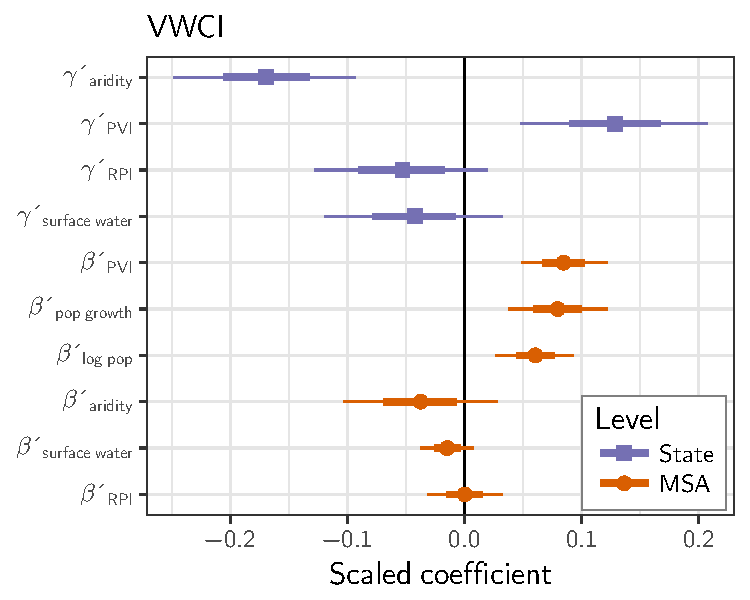
\includegraphics[width=0.8\linewidth]{figure/vwci_cat_plot-1}

}

\caption[Scaled regression coefficients for VWCI]{Scaled regression coefficients for VWCI: $\gamma$ refer to state-level regression coefficients and $\beta$ to MSA-level ones.
%Coefficients are scaled  so the value on the horizontal axis represents the approximate change in the probability $p_i$ of adopting an action, corresponding to a  two-standard-deviation change in the predictor when $p_i$ is around 0.5.
For a scaled coefficient of 0.1, a two-standard-deviation change in the predictor corresponds to VWCI changing by about 8 for a city with a VWCI of around 40. The points represent the median of the posterior, the thick lines the 66\% highest-density interval (HDI), and the thin lines the 95\% HDI. Coefficients are grouped by state vs. city level and then ordered within each group by absolute value of the median.}\label{fig:vwci_cat_plot}
\end{figure}


%
% req_reb_cat_plot
%
% jg_tex_chunk_hook

\begin{figure}[tbp]

{\centering 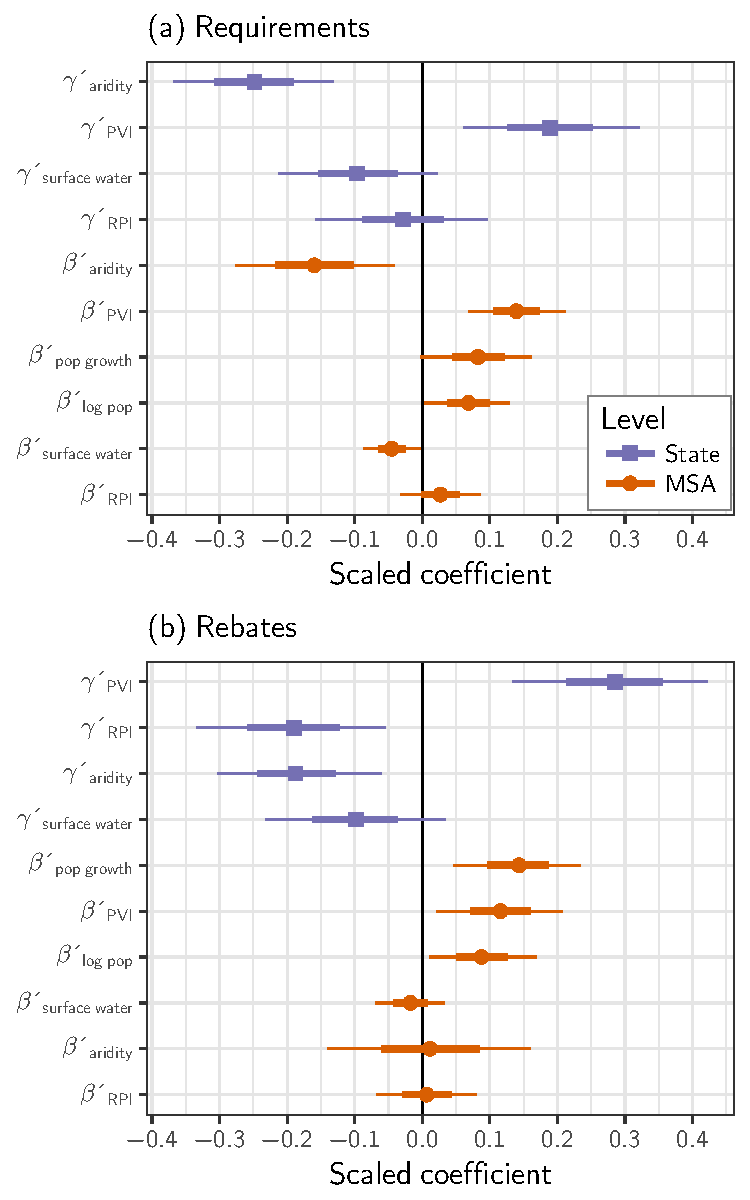
\includegraphics[width=0.8\linewidth]{figure/req_reb_cat_plot-1}

}

\caption[Scaled regression coefficients for conservation requirements and rebates]{Scaled regression coefficients for conservation requirements and rebates. For a scaled coefficient of 0.1, a two-standard-deviation change of the predictor corresponds to the number of requirements changing by about 3 for a city with around 16 requirements, and a the number of rebates changing by about 2 for a city with around 10 rebates.}\label{fig:req_reb_cat_plot}
\end{figure}


%
% req_cat_plot
%

%
% reb_cat_plot
%


States with more positive (Democratic-leaning) PVI have greater propensity to adopt conservation policies, as do MSAs whose PVI is greater (more likely to vote Democratic) than the rest of the state. States with drier climates (negative aridity)
also have greater propensity for conservation. MSAs with large and rapidly growing populations also tend to score higher on all three measures.

For all three conservation scores, the largest effects were for state-level, as opposed to MSA-level, characteristics, but the posterior distributions show considerable overlap so it is important not to over-interpret the ranking of coefficients.

Two differences that stand out among the three measures are that state-level variation in RPI and MSA-level variation in aridity each has ambiguous effects on total VWCI and different effects on requirements versus rebates: state-level RPI affects rebates more strongly than requirements and MSA-level variations in aridity affect requirements more strongly than rebates.

%
% vwci_residual_range
%

Regression residuals for VWCI range from $-14.9$ to~$+17.1$, with a root-mean-square value of $5.3$ (Figure~\ref{fig:vwci_residuals} and Table~\ref{tab:vwci_top_residuals}).
There is no indication of multicollinearity creating worrisome correlations among the coefficients (Figures.~S3--S5).
%
% vwci_residuals
%
% jg_tex_chunk_hook

\begin{figure}[tb]

{\centering 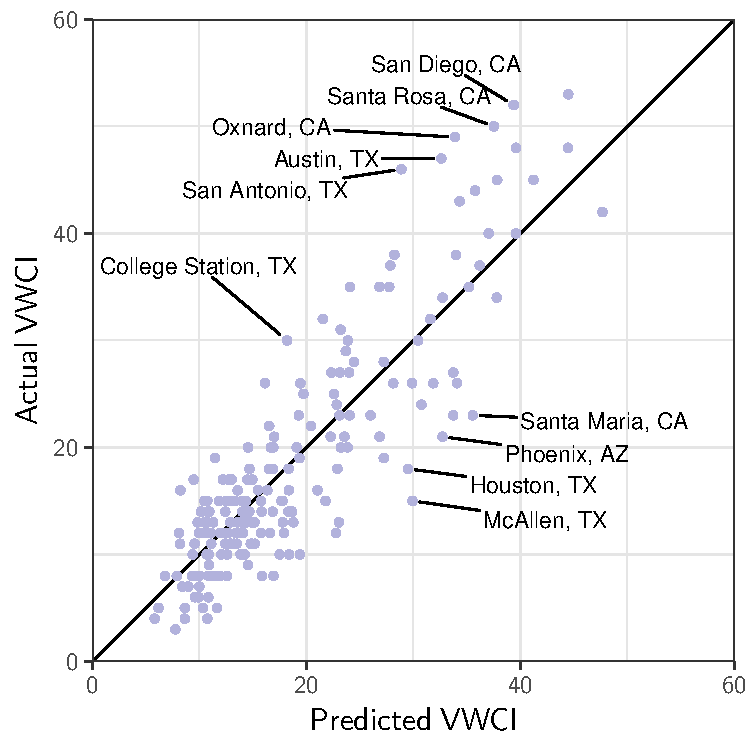
\includegraphics[width=0.8\linewidth]{figure/vwci_residuals-1}

}

\caption[Predicted versus actual VWCI]{Predicted versus actual VWCI. Cities with the ten largest residuals are labeled.}\label{fig:vwci_residuals}
\end{figure}


%
% vwci_top_residuals
%
% latex table generated in R 3.3.3 by xtable 1.8-2 package
% Mon Apr  3 17:22:34 2017
\begin{table}[tbp]
\centering
\caption{Cities with the ten largest residuals from VWCI regression.}
\label{tab:vwci_top_residuals}
\begin{tabular}{rlrrr}
  \hline
\multicolumn{1}{c}{ Rank } & \multicolumn{1}{c}{ City } & \multicolumn{1}{c}{ VWCI } & \multicolumn{1}{c}{ predicted VWCI } & \multicolumn{1}{c}{ residual } \\
  \hline
 1 & San Antonio, TX & 46 & 28.9 & 17.1 \\
   2 & Oxnard, CA & 49 & 33.9 & 15.1 \\
   3 & McAllen, TX & 15 & 29.9 & $-$14.9 \\
   4 & Austin, TX & 47 & 32.6 & 14.4 \\
   5 & San Diego, CA & 52 & 39.4 & 12.6 \\
   6 & Santa Maria, CA & 23 & 35.6 & $-$12.6 \\
   7 & Santa Rosa, CA & 50 & 37.5 & 12.5 \\
   8 & College Station, TX & 30 & 18.2 & 11.8 \\
   9 & Phoenix, AZ & 21 & 32.7 & $-$11.7 \\
  10 & Houston, TX & 18 & 29.5 & $-$11.5 \\
   \hline
\end{tabular}
\end{table}


\section{Discussion}

This analysis identifies distinguishing characteristics of cities across the contiguous United States that embrace water conservation policies, and allows us to differentiate state-level from MSA-level effects. We find that water conservation is driven both by characteristics of the physical environment and by political and demographic
%, and economic
characteristics of cities and states.

Our previous qualitative analysis of the 22~largest southwestern MSAs suggested that partisan differences over water conservation are more muted at the MSA-level than at the state and national level \citep{hess_drought_2016}, but while the quantitative analysis of that data showed that PVI played a large role, it could not distinguish state-level from MSA-level effects. Here, we find that for all three conservation scores (total VWCI, requirements only, and rebates only), PVI is important at both the state and MSA levels. The effect of PVI on all three conservation scores appears to be greater at the state level than at the MSA-level, but the posterior distributions of state-level and MSA-level coefficients overlap too much to permit much confidence in this ranking.

The state climate (aridity) shows clear effects that are consistent across all three conservation scores. The effects of variation in MSA-level aridity within a state on VWCI and rebates are much smaller, ambiguous, and consistent with zero. We interpret this as reflecting the fact that urban water supplies often draw from sources, such as river networks, watersheds, and aquifers, that cover large areas and which may be shared by many cities and many categories of users. However, aridity has a clear effect on requirements, with cities that are drier than the state average tending to adopt more requirements.

RPI measures the real purchasing power of per-capita personal income, adjusted for inflation and regional variations in the cost of living \citep{bea_rpp_methodology_2016}, and thus reflects prosperity. At the state level, greater RPI correlates with lower conservation scores on all three measures, but the effect is small and ambiguous (consistent with zero) for VWCI and requirements, whereas it is large and clearly nonzero for rebates. Perhaps this reflects greater political support for choosing rebates over requirements when households have less disposable income with which to pay for conservation actions. At the MSA-level, variations of RPI within a state have negligibly small effects, which are consistent with zero, on all three scores.

What emerges in the big picture is that cities in states with higher (more Democratic-leaning) PVI's and more arid climates tend to adopt more conservation measures, including more requirements and more rebates. State-level RPI does not have a clear effect on VWCI, but RPI appears to affect the composition of conservation policies, with lower RPI coreresponding to a greater reliance on rebates. Within a state, cities in MSAs with greater PVI than the state average and those with large and rapidly growing populations tend to adopt more total conservation measures, including more rebates and requirements. Variations in aridity from one MSA to another within a state do not have an appreciable effect on total VWCI, but they do affect the composition of policies, with MSAs whose climate is more arid than the state average tending to favor requirements over other conservation measures.

\citet{brown_politics_2016} report on detailed interviews with decision-makers from four cities, including
San Antonio and Phoenix, which have the largest and ninth-largest residuals, respectively
(Table~\ref{tab:vwci_top_residuals}). This merits some discussion: San Antonio has a low predicted VWCI in part because of its low (Republican-leaning) PVI. However, federal policy may have contributed to San Antonio having a much higher VWCI than predicted by our regression: San Antonio's options for increasing its water supply are constrained by the settlement of a lawsuit over endangered species, which requires the U.S. Fish and Wildlife Service to restrict withdrawals from the Edwards Aquifer \citep{brown_politics_2016}. Phoenix has a much lower water conservation index than predicted. One contributing factor may be the city's access to water from the Colorado River, by means of the Central Arizona Project, which significantly relieves the water stress that might be expected from the region's hydroclimatology \citep{brown_politics_2016}.

One should be cautious about using using qualitative data based on historical conditions to explain unusual observations or deviations from a model, but these two examples illustrate the rich complexity of water conservation policy and suggest that in future research, mixed-methods approaches can be valuable, combining statistical analyses with detailed case studies of selected cities to study both the patterns that represent what cities have in common and the distinctive individual characteristics of different cities.

In comparing the findings of this analysis to those of our previous preliminary analysis of the 22~largest MSAs in the Southwest, both studies identified PVI as a very important predictor of water conservation policies, but with its much smaller and less diverse sample, the previous study could not identify other effects after controlling for PVI, and it could not quantitatively distinguish state-level from MSA-level effects of PVI or other covariates. Here we observe clearly that variations in both environmental and societal characteristics at the state level are relevant to policy adoption; that within a state, variations from MSA to MSA of PVI, population, and population growth are consistently important; and that MSA-level variation in climate does not affect the number of conservation policies adopted, but affects the kinds of policies adopted.

\section{Conclusion}
An integrated perspective that draws on social science and natural science variables shows that the adoption of urban water conservation policies cannot be explained by considering only hydroclimatological factors, such as aridity and the surface water fraction. Societal variables, such as political leanings, are also important. This analysis finds that for the most part, hydroclimatological variables are important at the state level, but not at the MSA level, whereas PVI is important at both the state and MSA level.
Economic well-being has smaller and more ambiguous effects, but appears to affect which categories of conservation policies a city is likely to favor.
These results suggest that large, rapidly growing, and more politically liberal cities, and cities in arid and politically liberal states, will be more likely to adopt water conservation policies.
Policy rationales for water conservation and proposals for specific conservation measures would likely benefit from taking into account the complex mix of factors revealed by integrated social and natural science research.


\acknowledgments
This material is based upon work supported by the National Science Foundation under Grant \#EAR-1416964.
%, and by the U.S. Geological Survey, National Water-Use Information Program and the Lower Mississippi-Gulf Water Science Center project ``Water Conservation in American Cities.''
The authors thank Christopher Fonnesbeck for helpful discussions and suggestions.
All data used for this paper are properly cited and listed in the references or included in the supplementary information. The complete VWCI data set, together with the code (R scripts and Stan models) used for this analysis, will also be posted publicly on github prior to publication.
%
% Bibliography
\bibliography{gilligan_vwci_ef_2017}

\end{document}

